Graphs present a powerful abstraction for representing data and their internal relationships. The collection of data and the relationships among them, represented as graphs, have reached unmatched levels in recent years. These graphs are usually immense in scale, stemming from applications such as machine learning and social networks. \textit{Community detection} is an NP-hard problem in graph analytics with numerous applications in domains such as drug discovery, protein annotation, disease prediction, topic discovery, inferring land use, and criminal identification. Finding communities in graphs is a well-studied problem, where the primary objective is to identify groups of vertices that exhibit dense internal connections but sparse connections with the rest of the graph. These communities are intrinsic when identified based on network topology alone, without external attributes, and they are disjoint when each vertex belongs to only one community \cite{com-gregory10}.
\ignore{Finding communities in graphs is an NP-hard problem that tries to find inherent sets in a graph, where the vertices within a community are more strongly connected to each other than those outside. These communities find extensive applications in recommendation systems, targeted advertising, drug discovery, protein annotation, and topic discovery \cite{com-gregory10}.}
\ignore{Two popular heuristic-based algorithms for intrinsic and disjoint community detection are the \textit{Louvain} method \cite{com-blondel08} and the \textit{Label Propagation Algorithm (LPA)} \cite{com-raghavan07}. Communities are intrinsic when identified based on network topology alone, and are disjoint when each vertex belongs to only one community. Community detection algorithms use the modularity metric proposed by Newman et al. \cite{com-newman06} to measure the quality of the communities identified.}

One of the difficulties in the community detection problem is the lack of apriori knowledge on the number and size distribution of communities. Two popular heuristic-based approaches to community detection are the \textit{Louvain} method \cite{com-blondel08} and the \textit{Label Propagation Algorithm (LPA)} \cite{com-raghavan07}. Current work on community detection uses the modularity metric proposed by Newman et al. \cite{com-newman06} to measure the quality of the communities identified. Several recent studies show how to implement \Lou{} method and \LPA{} on modern architectures such as multi-core CPUs \cite{com-fazlali17}, GPUs \cite{com-cheong13}, CPU-GPU hybrid platforms \cite{com-bhowmick22}, distributed platforms \cite{com-ghosh18}, and the like. While the \textit{Louvain} algorithm obtains high-quality communities, we find it to be $2.3 - 14\times$ slower than \textit{LPA} (which obtains communities of lower quality by $3.0 - 30\%$).

With the data deluge\ignore{and ever-changing application requirements}, newer challenges are emerging. Many real-world graphs evolve with the insertion/deletion of edges/vertices. For efficiency reasons, one needs algorithms that update the results without re-computing from scratch. Such algorithms are known as \textit{dynamic algorithms}. Examples of parallel dynamic algorithms include those for dynamic graph coloring \cite{color-yuan17, color-bhattacharya18}, maintaining shortest routes \cite{path-zhang17, path-khanda21}, and updating centrality scores \cite{cent-shao20, cent-regunta21}.
\ignore{The collection of data and the relationships among them, represented as graphs, have reached unmatched levels in recent years.}
\ignore{With the data deluge and ever-changing application requirements, newer challenges are emerging. Many real-world graphs evolve with the insertion/deletion of edges/vertices. For efficiency reasons, one needs algorithms that update the results without re-computing from scratch. Such algorithms are known as \textit{dynamic algorithms}. Parallelizing dynamic graph algorithms is challenging due to the complexities of handling concurrency, optimizing data access, and reducing resource contention, and load imbalance. Further, in the parallel setting, processing a batch of updates is often an effective method as doing so offers scope for exploiting parallelism and minimizes computational effort compared to processing individual updates.}

Parallelizing dynamic graph algorithms is challenging due to the complexities of handling concurrency, optimizing data access, and reducing resource contention, and load imbalance. One popular approach to extract parallelism is the \textit{batch dynamic} setting, where one processes a batch of updates simultaneously. A batch update allows extraction of parallelism and minimizes the work performed compared to the setting where the updates are applied individually. Parallel algorithms have to be designed appropriately to benefit from such latent parallelism.

There is a pressing need for efficient parallel algorithms for community detection on large dynamic graphs. The goal of \textit{dynamic community detection} is to obtain high-quality communities while minimizing computation time. One does this by choosing a suitable algorithm, reusing old community membership of vertices, and processing only a small subset of the graph likely to be affected by changes. Note that if the subset of the graph identified as \textit{affected} is too small, we may end up with inaccurate communities, and if the subset is too large, we incur a significant computation time. Hence, one should look to identify the appropriate set of affected vertices. In addition, determining the vertices to be processed should have low overhead \cite{incr-ramalingam96}. Existing approaches either process all vertices (such as \textit{Naive-dynamic}), over/underestimate the set of affected vertices, and/or have high overhead (such as \textit{$\Delta$-screening} \cite{com-zarayeneh21}). The algorithm of Zarayeneh et al. \cite{com-zarayeneh21} suffers from identifying far too many vertices as affected, thereby requiring a large amount of work to identify the new communities.

One recent approach for dynamic community detection in the parallel setting is the work of Reidy and Bader \cite{com-riedy13}. While being a parallel batch dynamic algorithm, the work of Reidy and Bader \cite{com-riedy13} has a few limitations. They do not consider cascading changes to community labels on an update or study the quality of obtained communities. We summarize the state-of-the-art in Table \ref{tab:comparision}. From Table \ref{tab:comparision}, we note that there is a need for efficient parallel algorithms for community detection on dynamic graphs.

\ignore{Dynamic community detection algorithms aim to obtain communities on evolving graphs while minimizing computation time. One does this usually by choosing a suitable algorithm, reusing old community labels of vertices, and processing a subset of the graph likely to be affected by changes. However, a perusal of the extant literature on indicates a few shortcomings. Some of these algorithms, \cite{com-cordeiro16,com-meng16} do not outperform the static algorithms even for modest sized batch updates. Many of the reported algorithms \cite{com-zarayeneh21,OTHERS} are not designed in the parallel setting. Algorithms such as from \cite{com-aynaud10,com-cheong13} adapt the existing community labels and run an algorithm such as the Louvain algorithm on the entire graph. Often, this is unwarranted since not every vertex would need to change its community on the insertion/deletion of a few edges. Finally, there are algorithms such as from \cite{com-zarayeneh21,OTHERS} that identify a subset of vertices whose community labels are likely to change on the insertion/deletion of a few edges. However, as this set of vertices identified is large, the algorithm of Zaranayeh et al. \cite{com-zarayeneh21} incur a significant computation time. Table \ref{tab:compare} summarizes the above discussion. }

\ignore{We observe from Table \ref{tab:compare} that the problem of designing efficient parallel algorithms that update the community structures of an evolving graph is important. Ideally, the algorithm should identify a subset of the graph to be processed with a low overhead \cite{incr-ramalingam96}. If the identified subset is too small, we may end up with inaccurate communities and if it is too large, we incur a significant computation time.}




\subsection{Our Contributions}
\label{sec:contribution}

This paper addresses the design of a high-speed community detection algorithm in the batch dynamic setting (where multiple edge updates are processed simultaneously), and identifies communities of high quality while addressing the concerns mentioned above.

We start by discussing our optimized parallel implementations of the \textit{Louvain} and \textit{LPA} algorithms, determining suitable parameter settings and optimizing the original algorithm through experimentation with a variety of techniques. The combined optimizations significantly enhance the performance of the OpenMP-based \textit{Louvain} and \textit{LPA}, achieving completion times of $6.2$ seconds and $2.7$ seconds, respectively, on a single 64-core CPU, when processing an undirected web graph with $1.9$ billion edges. We have experimented with COPRA \cite{com-gregory10}, SLPA \cite{com-xie11}, and LabelRank \cite{com-xie13}, but found LPA \cite{com-raghavan07} to be the most performant, while yielding communities of equivalent quality.

We then discuss our \textit{Dynamic Frontier} approach that incrementally identifies an approximate set of affected vertices in the graph, given a batch of edge deletions and insertions, with low runtime overhead. We show how to combine our \textit{Dynamic Frontier} approach to existing static algorithms for community detection such as \textit{Louvain} and \textit{LPA}. We perform the parallel executions and experimentations on a shared-memory multi-core CPU platform.

We compare \textit{Dynamic Frontier} with two other dynamic appro-aches, the \textit{Naive-dynamic} approach, and the \textit{Dynamic $\Delta$-screening} approach. On a collection of 12 graphs from four different classes, our experiments indicate that the \textit{Dynamic Frontier} approach coupled with \Lou{} has a mean improved performance of $1.5\times$ compared to \textit{Naive-dynamic} \textit{Louvain}, while obtaining communities of the same quality. On the same collection of graphs, the \textit{Dynamic Frontier} approach coupled with \LPA{} has a mean improved performance of $10.0\times$ compared to \textit{Naive-dynamic} \textit{LPA}, again while obtaining communities of equivalent quality. The work presented by Zarayeneh et al. \cite{com-zarayeneh21} demonstrates improved performance of \textit{$\Delta$-screening} compared to \textit{Dynamo} \cite{com-zhuang19} and \textit{Batch} \cite{com-chong13}. As the \textit{Dynamic Frontier} approach outperforms \textit{$\Delta$-screening}, we expect similar gains compared to \textit{Dynamo} and \textit{Batch}.

Finally, we discuss our \textit{Dynamic Frontier} based \textit{Hybrid Louvain-LPA} that combines \textit{Static Louvain} and \textit{Dynamic Frontier} based \textit{LPA} into a hybrid dynamic algorithm. This allows it to leverage the strengths of both algorithms while overcoming their individual limitations. It offers a $7.5\times$ speedup over \textit{Dynamic Frontier} based \textit{Louvain}, while yielding communities of high quality. To our knowledge, no prior work has explored a similar hybrid approach. \footnote{For reproducibility, our source code is at \url{https://bit.ly/hipc23-174}}




\ignore{
This paper addresses the design of efficient \textit{parallel Louvain} algorithm in the \textit{batch dynamic} setting, where multiple edge updates are processed simultaneously. \ignore{It identifies communities of high quality while addressing the concerns mentioned above.}

We start by proposing our parallel \textit{Dynamic Frontier} approach. Given a batch update consisting of edge deletions or edge insertions, the \textit{Dynamic Frontier} approach incrementally identifies an approximate set of affected vertices in the graph with a low run time overhead. 

We show how to combine our \textit{Dynamic Frontier} approach with two parallel algorithms: the parallel \Lou{} and the parallel LPA. In addition to accepting the previous community membership of each vertex, our algorithm accepts the previous total edge weight of each vertex \kk{edge weight of each vertex is a bit confusing -- reword this phrase} as auxiliary information in order to improve scalability. HYBRID?

We compare \textit{Dynamic Frontier} with the \textit{$\Delta$-screening} approach. On a collection of 12 graphs from four different classes, our experiments \kk{on a xx-core AMD EPYC server} indicate that the \textit{Dynamic Frontier} approach coupled with \Lou{} has $20\times$, $2.1\times$ lower run time on average compared to \textit{Static} and \textit{$\Delta$-screening} \textit{Louvain} upto a batch size of $0.01 |E|$, while obtaining communities of the same quality. We then show that our algorithm achieves \su{good} community stability. Community stability is important because it will simplify the process of tracking of communities over time. Finally, we show that our algorithm has good scaling performance. \footnote{For reproducibility, our source code is at https://bit.ly/hipc23-174}. 


\ignore{Our algorithm only performs community detection in the full network at the first snapshot. In the following snapshots, the previous community structure is taken into account by applying the Louvain in a much smaller set of affected vertices.}

\ignore{Empirical results have demonstrated that the proposed dynamic version keeps most of the communities of the previous snapshot unchanged. The modified Louvain steps will only compute communities which are affected by addition or removal of nodes/edges. Small network changes resulted in better elapsed time executions.}

\ignore{Unlike the static Louvain, that may change significantly the way communities are obtained between snapshots (two runs in the snapshot lead to different solutions due its non-determinism). In the proposed algorithm, unaffected communities keep unchanged. Therefore, they preserve the same nodes and even the same community id between snapshots. Community stability is important because it will simplify the process of tracking of communities over time.}

%We start by discussing our optimized \textit{parallel implementation} of the \textit{Louvain} algorithm, determining suitable parameter settings and optimizing the original algorithm through experimentation with a variety of techniques. The combined optimizations significantly enhance the performance of the OpenMP-based Louvain, achieving completion times of $6.2$ seconds on a single 64-core CPU, when processing an undirected web graph with $1.9$ billion edges.

% The work in this paper makes two key contributions: (i) the dynamic frontier approach that allows for quick identification of a small set of affected vertices, and (ii) a hybrid approach that ensures the time required to identify the communities is low, and the quality of the communities identified is good.
}

\begin{table}
\setlength{\tabcolsep}{1pt}
\centering
\begin{tabular}{|l|l|l|l|l|l|l|} \hline
 & \cite{com-zarayeneh21} & \cite{com-zhuang19} & \cite{com-chong13} &  \cite{com-xie13} & \cite{com-riedy13} & {\bf This paper} \\ \hline
Parallel & $\times$ & $\times$ & $\times$ & $\times$ & $\checkmark$ & $\checkmark$ \\ \hline
Fully dynamic & $\checkmark$ & $\checkmark$ & $\checkmark$ & $\checkmark$ & $\checkmark$ & $\checkmark$ \\ \hline
Batch update & $\checkmark$ & $\checkmark$ & $\checkmark$ & $\checkmark$ & $\checkmark$ &  $\checkmark$ \\ \hline
\end{tabular}
\caption{Comparison of community detection algorithms.}
\label{tab:comparision}
\end{table}





%% - Use --- for a dash.
%% - Use ``camera-ready'' for quotes.
%% - Use {\itshape very} or \textit{very} for italicized text.
%% - Use \verb|acmart| or {\verb|acmart|} for mono-spaced text.
%% - Use \url{https://capitalizemytitle.com/} for URLs.
%% - Use {\bfseries Do not modify this document.} for important boldface details.
%% - Use \ref{fig:name} for referencing.

%% For a block of pre-formatted text: 
% \begin{verbatim}
%   \renewcommand{\shortauthors}{McCartney, et al.}
% \end{verbatim}

%% For a list of items:
% \begin{itemize}
% \item the ``ACM Reference Format'' text on the first page.
% \item the ``rights management'' text on the first page.
% \item the conference information in the page header(s).
% \end{itemize}

%% For a table:
% \begin{table}
%   \caption{Frequency of Special Characters}
%   \label{tab:freq}
%   \begin{tabular}{ccl}
%     \toprule
%     Non-English or Math&Frequency&Comments\\
%     \midrule
%     \O & 1 in 1,000& For Swedish names\\
%     $\pi$ & 1 in 5& Common in math\\
%     \$ & 4 in 5 & Used in business\\
%     $\Psi^2_1$ & 1 in 40,000& Unexplained usage\\
%   \bottomrule
% \end{tabular}
% \end{table}

%% For a full-width table:
% \begin{table*}
%   \caption{Some Typical Commands}
%   \label{tab:commands}
%   \begin{tabular}{ccl}
%     \toprule
%     Command &A Number & Comments\\
%     \midrule
%     \texttt{{\char'134}author} & 100& Author \\
%     \texttt{{\char'134}table}& 300 & For tables\\
%     \texttt{{\char'134}table*}& 400& For wider tables\\
%     \bottomrule
%   \end{tabular}
% \end{table*}


%% For inline math:
% \begin{math}
%   \lim_{n\rightarrow \infty}x=0
% \end{math},

%% For a numbered equation:
% \begin{equation}
%   \lim_{n\rightarrow \infty}x=0
% \end{equation}

%% For an unnumbered equation:
% \begin{displaymath}
%   \sum_{i=0}^{\infty} x + 1
% \end{displaymath}

%% For a figure:
% \begin{figure}[h]
%   \centering
%   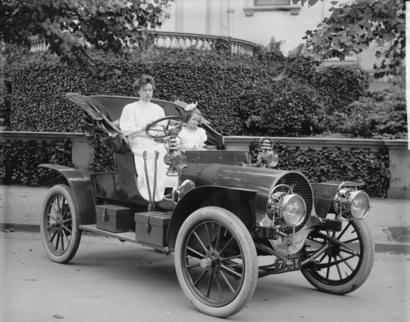
\includegraphics[width=\linewidth]{inc/sample-franklin}
%   \caption{1907 Franklin Model D roadster. Photograph by Harris \&
%     Ewing, Inc. [Public domain], via Wikimedia
%     Commons. (\url{https://goo.gl/VLCRBB}).}
%   \Description{A woman and a girl in white dresses sit in an open car.}
% \end{figure}

%% For a teaser figure.
% \begin{teaserfigure}
%   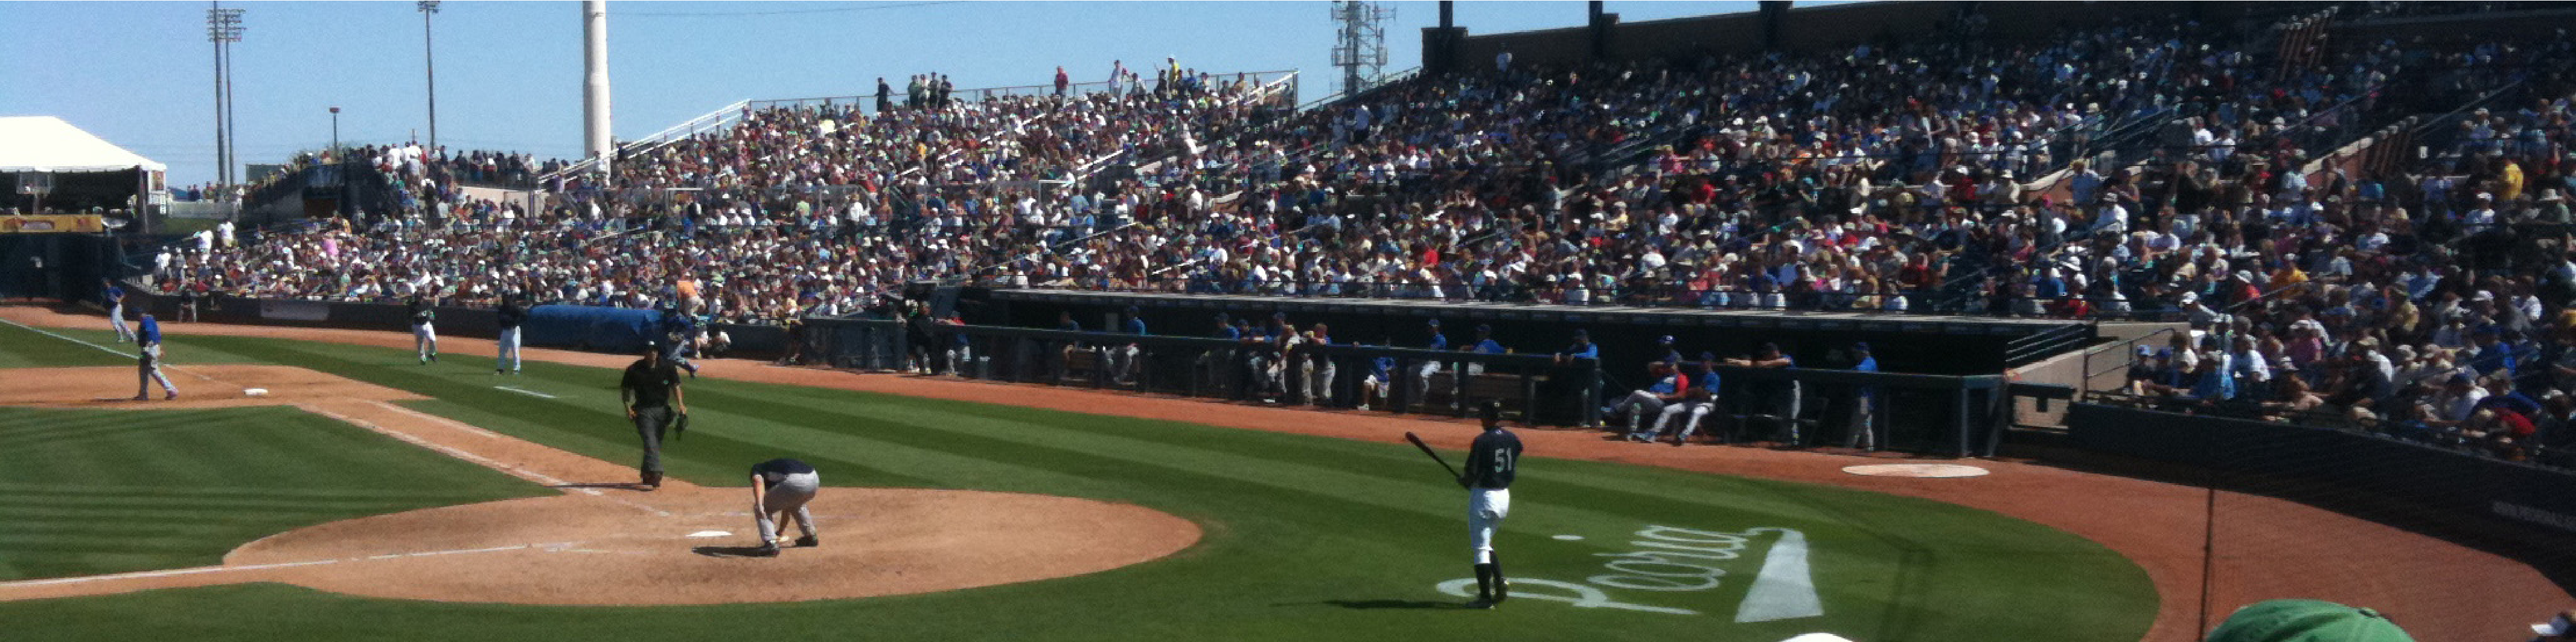
\includegraphics[width=\textwidth]{sampleteaser}
%   \caption{figure caption}
%   \Description{figure description}
% \end{teaserfigure}
